\documentclass[14pt]{extarticle}
\usepackage[utf8]{inputenc}
\usepackage[magyar]{babel}
\usepackage[section]{placeins}
\usepackage[a4paper, total={7in, 9in}]{geometry}
\usepackage{graphicx}
\graphicspath{ {../} }
\usepackage{fancyhdr}
\usepackage{hyperref}
\hypersetup{colorlinks,linkcolor=black,linktoc=section}
\pagestyle{fancyplain}
\fancyhf{}
\renewcommand{\headrulewidth}{0pt}

\begin{document}
	\begin{titlepage}
    \centering
    \vspace*{\fill}

    \vspace*{0.5cm}

    \huge\bfseries
    Jegyzőkönyv

    \vspace*{0.5cm}
	
	\sffamily\mdseries
    \large Adatkezelés XML környezetben
    
    \vspace{0.3cm}
    
    \normalsize Gyártó és Eladó folyamat

    \vspace*{\fill}
    
    \raggedleft
    Készítette: Korom Tamás\linebreak
    Neptun Kód: N7D1L5\linebreak
    Dátum: \today
    \end{titlepage}

    \newpage
    \tableofcontents
    \newpage
	\begin{normalsize}
		\section{Feladat leírás}
		\subsection{Feladat témája}
		\begin{normalsize}
			Az én féléves feladatom témája az Autó gyártó cégek és a velük kapcsolatban álló viszont eladók közötti kapcsolatot mutatja be. Az alap koncepció hogy vannak vevőink akik gyártóktól vásárolnak el autókat és ezeket fogjuk mi nyilván tartani. Ezek kapcsolati összefüggéseket a későbbiekben foglalkozni fogunk vele. Ez a kis adatbázis rendszer az alábbi dolgokat tárolja. Eladó adait, Gyártó adait, Dolgozó adait melyik gyárban dolgozik, melyik autót melyik gyárban gyártják és milyen motor van az adott gépjármű típusban.
		\end{normalsize}
		\subsection{Egyedek leírása}
		\begin{normalsize}
			Az eladó, gyártó, kocsi, és motor egyedek csak a legfontosabb alapvető információkat tartalmazzák, hogy a beadandó kritériumainak megfeleljenek.\newline
			Itt a dolgozó ami érdekes mert ez az egy egyed tartalmaz csak összetett és több értékű adatmezőt, ezek a mezők a többi egyednél nem találhatóak meg.\newline
			
			Az eladó csak az alap információkat tartalmazza ezek az alábbiak: Viszont eladó neve, Címe, adószáma, Tulajdonos neve, ID.\newline
			A gyártó is csak alapinformációkat tartalmaz ezek az alábbiak: Gyártó neve, Tulajdonosa, ID, adószáma, Cím.\newline
			A dolgozó már tartalmaz összetetteb adat típusokat is az alábbi mezőket tartalmazza ez az egyed: DID, születési dátum, Neve, Cím (ami egy összetett adat típus), Telefonszám(több értékü mert 1 dolgozónak lehet több telefonszáma is akár).\newline
			Kocsi itt is csak alap értékekkel találkozunk: KID, neve, hajtása, típusa.\newline
			Motor itt is csak nagyon alapvető dolgok szerepelnek: MID, motor űrtartalma, Motor típusa, Teljesítménye.\newline
			
			Ezek lennének az egyedek megvalósítva a feladat további részében.
			
		\end{normalsize}
		\subsection{Kapcsolatok leírása}
		\begin{normalsize}
			\bfseries Eladó és Gyártó közötti kapcsolatok: \mdseries Az eladó és a gyártó között \bfseries Több-Több \mdseries kapcsolat van mert 1 gyártó több eladóval is kapcsolatban lehet, és egy eladó több gyártóval is dolgozhat együtt.\newline
			\bfseries Gyártó és Dolgozó közötti kapcsolatok: \mdseries A gyártó és a dolgozó közötti kapcsolat abban fog meg nyilvánulni hogy \bfseries Egy-Több \mdseries kapcsolat ezt beláthatjuk mert egy dolgozó csak 1 gyárban tud dolgozni csak, de 1 gyárban dolgozhat több dolgozó is akár, ha nem egyéni vállalkozásról van szó, egy ilyen autógyárban általában többen dolgoznak mint 1 fő.\newline
			\bfseries Gyártó és Kocsi közötti kapcsolatok:\mdseries Itt is ugyanaz a helyzeti mint a dolgozó és a gyártó közötti kapcsolat itt is 1 gyárban több típusú de egy azon márkájú kocsit gyártanak de 1 féle típusú márkáju autót 1 gyárban gyártanak le. Szóval itt is \bfseries Egy-Több \mdseries kapcsolatról van szó.\newline
			\bfseries Kocsi és Motor közötti kapcsolatok: \mdseries Itt a kocsi és a motor közötti kapcsolat itt ott mutatkozik be hogy 1 féle típusú autóba csak 1 féle motor kerülhet más nem. Szóval ebből adódik hogy \bfseries Egy-Egy  \mdseries kapcsolatról van szó. 
		\end{normalsize}
		\section{ER model}
		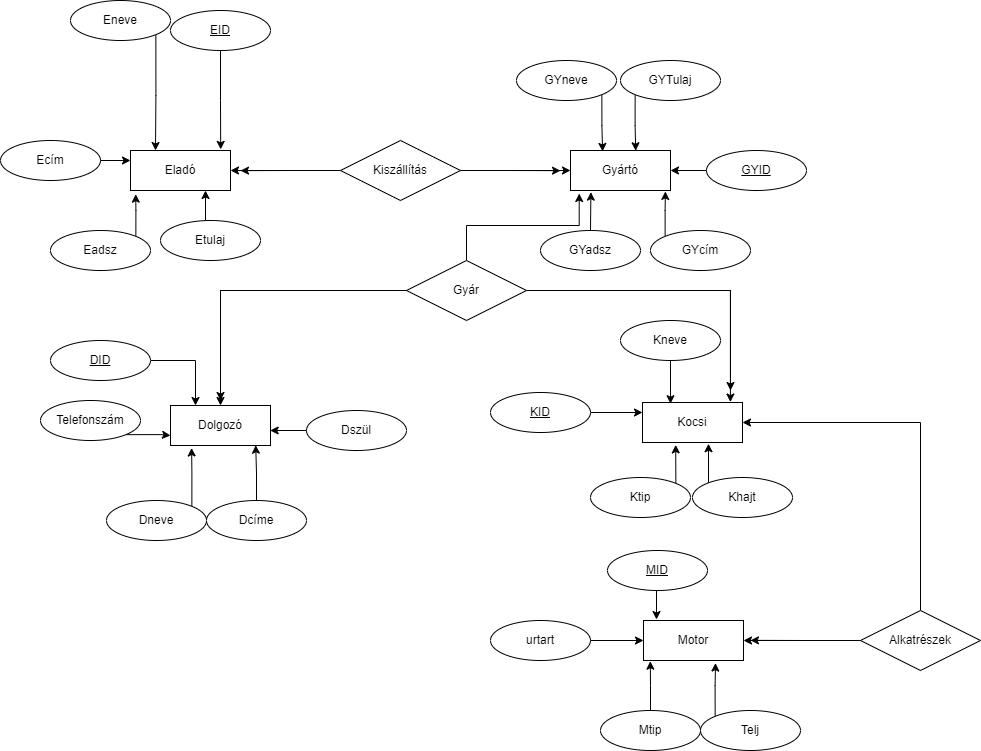
\includegraphics[scale=0.55]{N7D1L5_ER}
		Ígyekeztem minél jobban elkészíteni az ER modelt ahogy lehetet a követelményeknek megfelelően. Ez megtalálható a Githubon $N7D1L5_ER$ és png file-ként itt csak egy kicsinyitett verzió található meg.
		\section{XDM model}
		Az ER model segítsége alapján próbáltam meg össze rakni az XMD modelt ami nagyon széles lett és így nagyon le kellet kicsinyíteni de ezt a modelt is meglehet találni a githubon $XDMN7D1L5$ és png file-ként.
		\begin{center}
			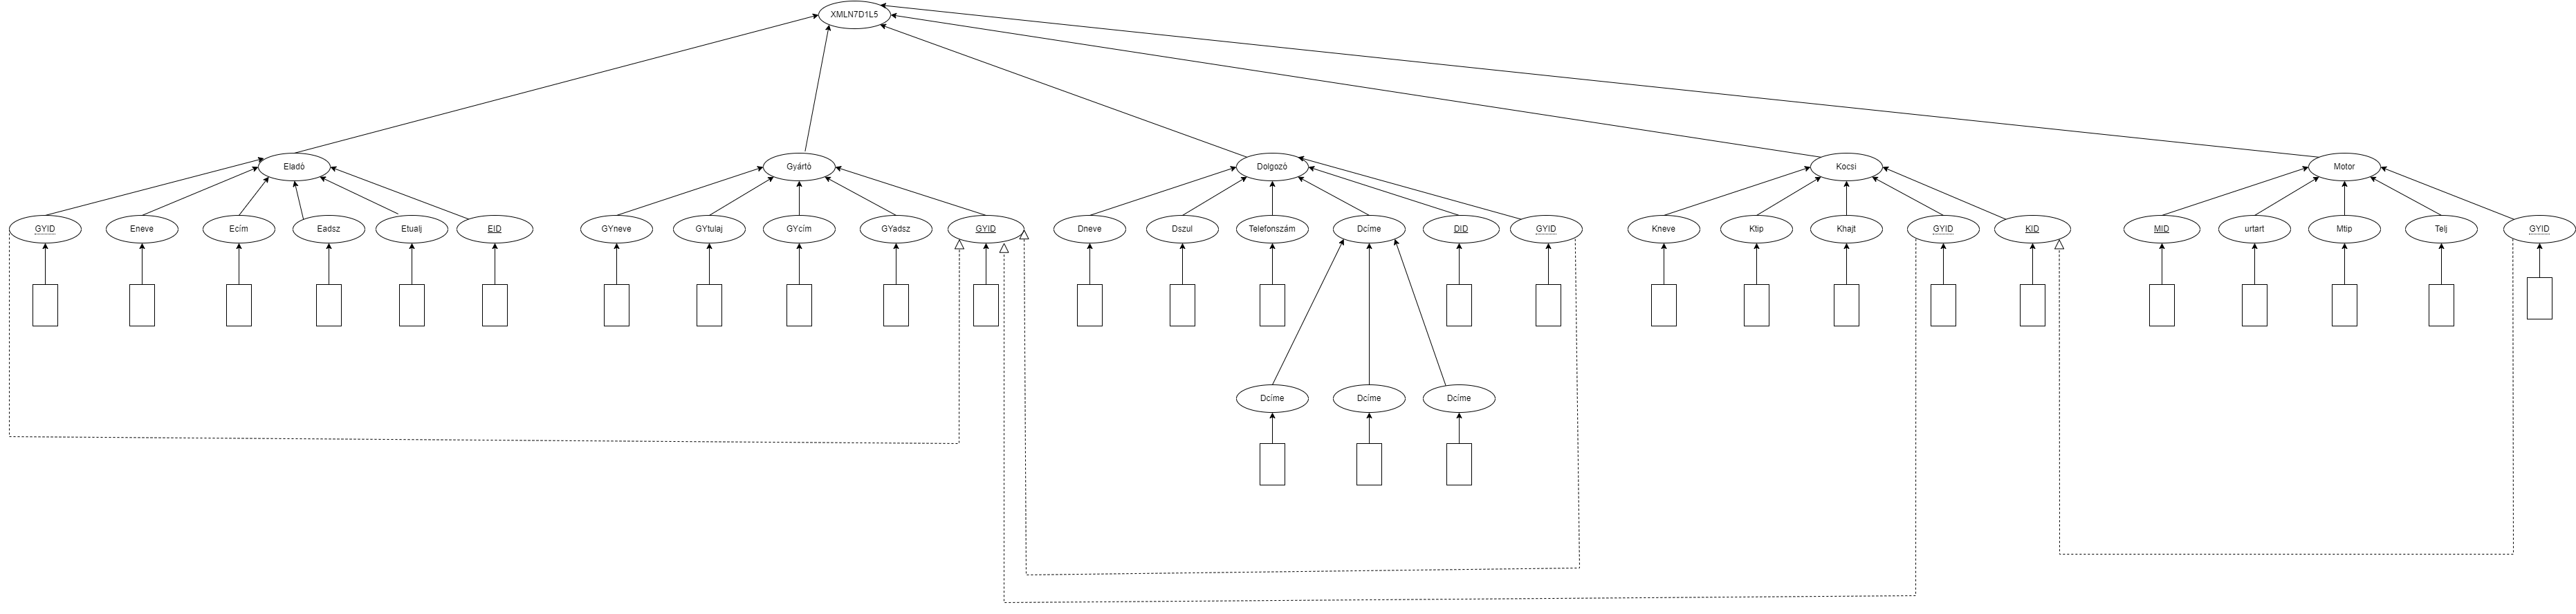
\includegraphics[scale=0.215, angle=270]{XDMN7D1L5}
		\end{center}
		\section{XML dokumentum}
		\begin{verbatim}
			<?xml version="1.0" encoding="UTF-8"?>
<!DOCTYPE xml>

<kocsik xmlns:xsi="https://w3.org/2001/XMLSchema-instance" 
	xsi:noNamespaceSchemaLocation="XMLN7D1L5.xsd">
    <elado EID="1">
        <etulaj>Kis Erno</etulaj>
        <eadsz>16516651</eadsz>
        <ecim>Miskolc, Kis Erno utca 2</ecim>
        <eneve>Muscle Car</eneve>
    </elado>
    <elado EID="2">
        <etulaj>Kovacs Janos</etulaj>
        <eadsz>16546516</eadsz>
        <ecim>Miskolc, Ujgyori Piac 10</ecim>
        <eneve>Citroen</eneve>
    </elado>
    <elado EID="3">
        <etulaj>Kis Tibor</etulaj>
        <eadsz>455464565</eadsz>
        <ecim>Miskolc, Kis Tabornok utca 7a</ecim>
        <eneve>Lada</eneve>
    </elado>

    <kiszallitas GYID="1" EID="1"/>
    <kiszallitas GYID="2" EID="3"/>
    <kiszallitas GYID="3" EID="02"/>

    <gyarto GYID="1">
        <gyneve>Dodge</gyneve>
        <gytulaj>Kis Pista</gytulaj>
        <gycim>Budapest, Nagy korut 3</gycim>
        <gyadsz>6541651566</gyadsz>
    </gyarto>
    <gyarto GYID="2">
        <gyneve>Peugeot</gyneve>
        <gytulaj>Kis Bence</gytulaj>
        <gycim>Kapuvar, Nagy korut 3</gycim>
        <gyadsz>6544651651566</gyadsz>
    </gyarto>
    <gyarto GYID="3">
        <gyneve>Ford</gyneve>
        <gytulaj>Kis Ferenc</gytulaj>
        <gycim>Debrecen, Nagy Pista utca 3</gycim>
        <gyadsz>6541651784566</gyadsz>
    </gyarto>

    <gyar GYID="1" DID="1"/>
    <gyar GYID="3" DID="3"/>
    <gyar GYID="2" DID="2"/>

    <dolgozo DID="1">
        <dneve>Jozsef Atilla</dneve>
        <dcime>
            <irsz>1007</irsz>
            <varos>Budapest</varos>
            <utca>Kassai utca 2</utca>
        </dcime>
        <dszul>1987.12.01</dszul>
        <dtel>36204546516</dtel>
	<dtel>3620524516</dtel>
	<dtel>3620728516</dtel>
    </dolgozo>
    <dolgozo DID="2">
        <dneve>Fekete Peter</dneve>
        <dcime>
            <irsz>7400</irsz>
            <varos>Kaposvár</varos>
            <utca>Szerencsi utca 2</utca>
        </dcime>
        <dszul>1987.12.01</dszul>
        <dtel>36208976516</dtel>
	<dtel>36207796516</dtel>
    </dolgozo>
    <dolgozo DID="3">
        <dneve>Petofi Sandor</dneve>
        <dcime>
            <irsz>3527</irsz>
            <varos>Miskolc</varos>
            <utca>Soltész Nagy Kálmán utca 7</utca>
        </dcime>
        <dszul>1987.12.01</dszul>
        <dtel>36204546516</dtel>
    </dolgozo>

    <gyar GYID="1" KID="1"/>
    <gyar GYID="2" KID="2"/>
    <gyar GYID="3" KID="3"/>


    <auto KID="1">
        <kneve>Dodge Challanger Demon</kneve>
        <ktip>Sedan</ktip>
        <khajt>Hatso</khajt>
    </auto>
    <auto KID="2">
        <kneve>Peugeot 403</kneve>
        <ktip>Sedan</ktip>
        <khajt>Elso</khajt>
    </auto>
    <auto KID="3">
        <kneve>Ford Raptor</kneve>
        <ktip>Terep</ktip>
        <khajt>Ossz</khajt>
    </auto>

    <alkatresz KID="1" MID="1"/>
    <alkatresz KID="2" MID="2"/>
    <alkatresz KID="3" MID="3"/>

    <motor MID="1">
        <urtart>6400</urtart>
        <mtip>Benzin</mtip>
        <telj>1000</telj>
    </motor>
    <motor MID="2">
        <urtart>1400</urtart>
        <mtip>Dizel</mtip>
        <telj>150</telj>
    </motor>
    <motor MID="3">
        <urtart>3200</urtart>
        <mtip>Benzin</mtip>
        <telj>380</telj>
    </motor>
</kocsik>
		\end{verbatim}
		\section{XML schema}
		\begin{verbatim}
			<?xml version="1.0" encoding="UTF-8"?>

<xs:schema xmlns:xs="http://www.w3.org/2001/XMLSchema" elementFormDefault="qualified" attributeFormDefault="unqualified">

<xs:element name="kocsik" type="kocsiTipus">
		<xs:key name="K1">
				<xs:selector xpath="elado" />
				<xs:field xpath="@id" />
			</xs:key>
			<xs:key name="K2">
				<xs:selector xpath="gyarto" />
				<xs:field xpath="@id" />
			</xs:key>
			<xs:key name="K3">
				<xs:selector xpath="dolgozo" />
				<xs:field xpath="@id" />
			</xs:key>
			<xs:key name="K4">
				<xs:selector xpath="auto" />
				<xs:field xpath="@id" />
			</xs:key>
			<xs:key name="K5">
				<xs:selector xpath="motor" />
				<xs:field xpath="@id" />
			</xs:key>
			
			<xs:keyref refer="K1" name="refK1">
				<xs:selector xpath="kiszallitas" />
				<xs:field xpath="@GYID" />
			</xs:keyref>
			<xs:keyref refer="K2" name="refK2_1">
				<xs:selector xpath="kiszallitas" />
				<xs:field xpath="@EID" />
			</xs:keyref>
			<xs:keyref refer="K2" name="refK2_2">
				<xs:selector xpath="gyar" />
				<xs:field xpath="@GYID" />
			</xs:keyref>
			<xs:keyref refer="K3" name="refK3_1">
				<xs:selector xpath="gyar" />
				<xs:field xpath="@DID" />
			</xs:keyref>
			<xs:keyref refer="K3" name="refK3_2">
				<xs:selector xpath="gyar" />
				<xs:field xpath="@GYID" />
			</xs:keyref>
			<xs:keyref refer="K4" name="refK4_1">
				<xs:selector xpath="gyar" />
				<xs:field xpath="@KID" />
			</xs:keyref>
			<xs:keyref refer="K4" name="refK4_2">
				<xs:selector xpath="alkatresz" />
				<xs:field xpath="@KID" />
			</xs:keyref>
			<xs:keyref refer="K5" name="refK5_1">
				<xs:selector xpath="alkatresz" />
				<xs:field xpath="@MID" />
			</xs:keyref>
		</xs:element>
			
			<xs:complexType name="kocsiTipus">
				<xs:sequence>
					<xs:element name="elado" type="eladoTipus" minOccurs="0" maxOccurs="100"/> 
					<xs:element name="kiszallitas" type="kiszallitasTipus" minOccurs="0" maxOccurs="100"/>
					<xs:element name="gyarto" type="gyartoTipus" minOccurs="0" maxOccurs="100"/>
					<xs:element name="gyar" type="gyarTipusd" minOccurs="0" maxOccurs="100"/>
                    <xs:element name="gyar" type="gyarTipusk" minOccurs="0" maxOccurs="100"/>
					<xs:element name="dolgozo" type="dolgozoTipus" minOccurs="0" maxOccurs="100"/>
					<xs:element name="kocsi" type="kocsiTipus" minOccurs="0" maxOccurs="100"/>
					<xs:element name="alkatresz" type="alkatreszTipus" minOccurs="0" maxOccurs="100"/>
					<xs:element name="motor" type="motorTipus" minOccurs="0" maxOccurs="100"/>
				</xs:sequence>
			</xs:complexType>
		
			
			<xs:complexType name="eladoTipus">
				<xs:sequence>
					<xs:element name="Etulaj" type="xs:string"/>
					<xs:element name="Eadsz" type="xs:unsignedLong"/>
					<xs:element name="Ecim" type="xs:string"/>
                    <xs:element name="Eneve" type="xs:string"/>
				</xs:sequence>
				<xs:attribute name="EID" type="xs:string" use="required"/> 
			</xs:complexType>
			
			<xs:complexType name="kiszallitasTipus">
				<xs:attribute name="EID" type="xs:string" use="required"/> 
				<xs:attribute name="GYID" type="xs:string" use="required"/>
			</xs:complexType>
			
			<xs:complexType name="gyartoTipus">
				<xs:sequence>
					<xs:element name="gyneve" type="xs:string"/>
					<xs:element name="gytulaj" type="xs:string"/>
                    <xs:element name="gycim" type="xs:string"/>
					<xs:element name="gyadsz" type="xs:unsignedLong"/>
				</xs:sequence>
                <xs:attribute name="GYID" type="xs:string" use="required"/>
			</xs:complexType>
			
			<xs:complexType name="gyarTipusd">
				<xs:attribute name="GYID" type="xs:string" use="required"/> 
				<xs:attribute name="DID" type="xs:string" use="required"/>
			</xs:complexType>

            <xs:complexType name="gyarTipusk">
				<xs:attribute name="GYID" type="xs:string" use="required"/> 
				<xs:attribute name="KID" type="xs:string" use="required"/>
			</xs:complexType>
			
			<xs:complexType name="dolgozoTipus">
				<xs:sequence>
					<xs:element name="dneve" type="xs:string"/>
					<xs:element name="dtel" type="xs:string"/>
					<xs:element name="dcime" type="xs:lakhely"/>
					<xs:element name="dszul" type="xs:string"/>
				</xs:sequence>
				<xs:attribute name="DID" type="xs:string" use="required"/> 
			</xs:complexType>

			<xs:complexType name="lakhelyTipus">
				<xs:sequence>
					<xs:element name="varos" type="xs:string"/>
					<xs:element name="utca" type="xs:string"/>
					<xs:element name="irsz" type="xs:string"/>
				</xs:sequence>
			</xs:complexType>
			
			<xs:complexType name="kocsiTipus">
				<xs:sequence>
					<xs:element name="kneve" type="xs:string"/>
					<xs:element name="ktip" type="xs:string"/>
					<xs:element name="khajt" type="xs:string"/>		
				</xs:sequence>
				<xs:attribute name="KID" type="xs:string" use="required"/> 
			</xs:complexType>

            <xs:complexType name="alkatreszTipus">
				<xs:attribute name="KID" type="xs:string" use="required"/> 
				<xs:attribute name="MID" type="xs:string" use="required"/>
			</xs:complexType>
			
			<xs:complexType name="motorTipus">
				<xs:sequence>
					<xs:element name="urtart" type="xs:unsignedLong"/>
					<xs:element name="mtip" type="xs:string"/>
                    <xs:element name="telj" type="xs:unsignedLong"/>
				</xs:sequence>
                <xs:attribute name="MID" type="xs:string" use="required"/>
			</xs:complexType>
			
</xs:schema>
		\end{verbatim}
		\section{DOM read}
		\subsection{DOM read leírás}
		\begin{normalsize}
			A DOM read beolvassa az \bfseries\itshape XMLN7D1L5.xml \mdseries\upshape dokumentumunkat és a beolvasott adatokat pedig kiírja a console-ra, ezen kivűl semmi különleges dolgot nem csinál.
		\end{normalsize}
		\subsection{DOM read Java kód}
		\small
		\begin{verbatim}
			package ReadN7D1L5;

import java.io.File;
import java.io.IOException;
import java.util.ArrayList;

import javax.xml.parsers.DocumentBuilder;
import javax.xml.parsers.DocumentBuilderFactory;
import javax.xml.parsers.ParserConfigurationException;

import org.w3c.dom.Document;
import org.w3c.dom.Element;
import org.w3c.dom.Node;
import org.w3c.dom.NodeList;
import org.xml.sax.SAXException;

public class READ_N7D1L5 {

	public static void main(String[] args) {
		
		
		//Az esetleges keletkezõ hibák lekezelése try-catch blokkban
		try {
//Az olvasandó fájl megadása
			 File xmlFile = new File("XMLN7D1L5.xml");
			 
//Az XML fájl átalakítása DOM objektumokká
		        DocumentBuilderFactory factory = DocumentBuilderFactory.newInstance();
		        DocumentBuilder dBuilder = factory.newDocumentBuilder();
		        Document doc = dBuilder.parse(xmlFile);
// Node-ok normalizálása
		        doc.getDocumentElement().normalize();
//A gyökér elem nevének kiolvasása és kiíratása konzolra		        
		        System.out.println("Gyökér elem: " + doc.getDocumentElement().getNodeName());
//A gyökér elem alatt fellelhetõ gyermek/testvér elemek listába illesztése
		        NodeList nList1 = doc.getElementsByTagName("elado");
		        NodeList nList2 = doc.getElementsByTagName("kiszallitas");
		        NodeList nList3 = doc.getElementsByTagName("gyarto");
		        NodeList nList4 = doc.getElementsByTagName("gyar");
		        NodeList nList5 = doc.getElementsByTagName("dolgozo");
		        NodeList nList6 = doc.getElementsByTagName("auto");
		        NodeList nList7 = doc.getElementsByTagName("alkatresz");
		        NodeList nList8 = doc.getElementsByTagName("motor");
		        System.out.println("----------------------------------------");

//Ciklus segítségével végignézzük az aktuális node lista elemeit
		        for (int i = 0; i < nList1.getLength(); i++) {
//Az egyes lista elemeket meghatározzuk node ként
		            Node nNode = nList1.item(i);
//Ha egyezést talál akkor Kiírjuk az adott elemhez tartozó nevet és adatokat is
		            if (nNode.getNodeType() == Node.ELEMENT_NODE) {
		   //A node-ot elemként definiáljuk
		            	Element elem = (Element) nNode;

		                System.out.println("\nAktuális elem: " + nNode.getNodeName());
		        // Az aktuális elemhez tartozó aazonosító letárolása egy String adattípusban
		                String id = elem.getAttribute("EID");
		        // Az adott elem gyermekelem értékének eltárolása String adattíõusban
		                Node node1 = elem.getElementsByTagName("Etulaj").item(0);
		                String nev = node1.getTextContent();
		                
		                Node node2_1 = elem.getElementsByTagName("Eadsz").item(0);
		                Node node2_2 = elem.getElementsByTagName("Ecim").item(0);
		                Node node2_3 = elem.getElementsByTagName("Eneve").item(0);
		                String ado = node2_1.getTextContent();
						String cim = node2_2.getTextContent();
		                String Eneve = node2_3.getTextContent();

		                // Az eltárolt értékek kiíratása
		                System.out.println("Elado ID-ja: " + id);
						System.out.println("Tulaj: " + nev);
		                System.out.println("Adoszama: " + ado);
		                System.out.println("Cime: " + cim);
		                System.out.println("Eneve: "+ Eneve);

		            }
		        }
// A továbbiakban minden listához ezt a megoldást alkalmazzuk		        
		        for (int i = 0; i < nList2.getLength(); i++) {
		            Node nNode = nList2.item(i);

		            if (nNode.getNodeType() == Node.ELEMENT_NODE) {
		                Element elem = (Element) nNode;

		                System.out.println("\nAktuális elem: " + nNode.getNodeName());

		                String id1 = elem.getAttribute("GYID");
		                String id2 = elem.getAttribute("EID");

		                System.out.println("Gyarto ID-ja: " + id1);
		                System.out.println("Elado ID-JA: " + id2);

		            }
		        }
		        
		        for (int i = 0; i < nList3.getLength(); i++) {
		            Node nNode = nList3.item(i);

		            if (nNode.getNodeType() == Node.ELEMENT_NODE) {
		                Element elem = (Element) nNode;

		                System.out.println("\nAktuális elem: " + nNode.getNodeName());

		                String id = elem.getAttribute("GYID");

		                Node node1 = elem.getElementsByTagName("gyneve").item(0);
		                String gyneve = node1.getTextContent();
		                
		                Node node2 = elem.getElementsByTagName("gytulaj").item(0);
		                String gytulaj = node2.getTextContent();
		                
		                Node node3 = elem.getElementsByTagName("gycim").item(0);
		                String gycim = node3.getTextContent();
		                
		                Node node4 = elem.getElementsByTagName("gyadsz").item(0);
		                String gyadsz = node4.getTextContent();


		                System.out.println("Könyv ID-ja: " + id);
		                System.out.println("Cím: " + gyneve);
		                System.out.println("Ár: "+gytulaj);
		                System.out.println("Szerző: "+gycim);
		                System.out.println("Oldalszám: "+gyadsz);
			            }
		        }
		        
		        for (int i = 0; i < nList4.getLength(); i++) {
		            Node nNode = nList4.item(i);

		            if (nNode.getNodeType() == Node.ELEMENT_NODE) {
		                Element elem = (Element) nNode;

		                System.out.println("\nAktuális elem: " + nNode.getNodeName());

		                String id2 = elem.getAttribute("GYID");
		                String id3 = "";
		                if(elem.getAttribute("DID") == "") {
		                	id3 = elem.getAttribute("KID");
		                	System.out.println("Gyar ID-ja: " + id2);
			                System.out.println("Kocsi ID-ja: " + id3);
			                }
		                else {
		                	id3 = elem.getAttribute("DID");
		                	System.out.println("Gyar ID-ja: " + id2);
			                System.out.println("Dolgozo ID-ja: " + id3);
		                }
		            }
		        }
		        
		        for (int i = 0; i < nList5.getLength(); i++) {
		            Node nNode = nList5.item(i);

		            if (nNode.getNodeType() == Node.ELEMENT_NODE) {
		                Element elem = (Element) nNode;

		                System.out.println("\nAktuális elem: " + nNode.getNodeName());

		                String id = elem.getAttribute("DID");

		                Node node1 = elem.getElementsByTagName("dneve").item(0);
		                String nev = node1.getTextContent();
		                
		                Node node2_1 = elem.getElementsByTagName("irsz").item(0);
		                String irsz = node2_1.getTextContent();
		                Node node2_2 = elem.getElementsByTagName("varos").item(0);
		                String varos = node2_2.getTextContent();
		                Node node2_3 = elem.getElementsByTagName("utca").item(0);
		                String utca = node2_3.getTextContent();
		                Node node3 = elem.getElementsByTagName("dszul").item(0);
		                String dszul = node3.getTextContent();
		                ArrayList<String> tel = new ArrayList<String>();
		                for(int j = 0; j < elem.getElementsByTagName("dtel").getLength(); j++) {
		                	Node node4 = elem.getElementsByTagName("dtel").item(j);
		                	tel.add(node4.getTextContent());
		                }
		                
		                System.out.println("Dolgozo ID-ja: " + id);
		                System.out.println("Név: " + nev);
		                System.out.println("Tel: "+tel);
		                System.out.println("Irsz: "+irsz);
		                System.out.println("varos: "+varos);
		                System.out.println("Utca: "+utca);
		                System.out.println("Született: "+dszul);

		            }
		        }
		        
		        for (int i = 0; i < nList6.getLength(); i++) {
		            Node nNode = nList6.item(i);

		            if (nNode.getNodeType() == Node.ELEMENT_NODE) {
		                Element elem = (Element) nNode;

		                System.out.println("\nAktuális elem: " + nNode.getNodeName());

		                String id = elem.getAttribute("KID");

		                Node node1 = elem.getElementsByTagName("kneve").item(0);
		                String nev = node1.getTextContent();
		                Node node2 = elem.getElementsByTagName("ktip").item(0);
		                String tip = node2.getTextContent();
		                Node node3 = elem.getElementsByTagName("khajt").item(0);
		                String hajt = node3.getTextContent();		             
		                
		                System.out.println("Kocsi ID-ja: " + id);
		                System.out.println("Név: " + nev);
		                System.out.println("Tel: "+tip);
		                System.out.println("Címe: "+hajt);

		            }
		        }
		        
		        for (int i = 0; i < nList7.getLength(); i++) {
		            Node nNode = nList7.item(i);

		            if (nNode.getNodeType() == Node.ELEMENT_NODE) {
		                Element elem = (Element) nNode;

		                System.out.println("\nAktuális elem: " + nNode.getNodeName());

		                String id2 = elem.getAttribute("KID");
		                String id3 = elem.getAttribute("MID");
  
		                System.out.println("Kocsi ID-ja: " + id2);
			            System.out.println("Motor ID-ja: " + id3);

		            }
		        }
		        
		        for (int i = 0; i < nList8.getLength(); i++) {
		            Node nNode = nList8.item(i);

		            if (nNode.getNodeType() == Node.ELEMENT_NODE) {
		                Element elem = (Element) nNode;

		                System.out.println("\nAktuális elem: " + nNode.getNodeName());

		                Node node1 = elem.getElementsByTagName("urtart").item(0);
		                String urtart = node1.getTextContent();
		                Node node2 = elem.getElementsByTagName("mtip").item(0);
		                String mtip = node2.getTextContent();
		                Node node3 = elem.getElementsByTagName("telj").item(0);
		                String telj = node3.getTextContent();	

		                System.out.println("Termék ID-ja: " + urtart);
		                System.out.println("Gyártó ID-ja: " + mtip);
		                System.out.println("Termék ID-ja: " + telj);

		            }
		        }
			
		}catch(SAXException sxe) {
			sxe.printStackTrace();
		}catch(ParserConfigurationException pe) {
			pe.printStackTrace();
		}catch(IOException ioe) {
			ioe.printStackTrace();
		}

	}



}

		\end{verbatim}
		\section{DOM modify}
		\subsection{DOM modify leírás}
		\begin{normalsize}
			A DOM modify itt valamilyen feltétel hatására fogjuk majd megváltoztatni az XML dokumentum egyik node-jának az értékét, vagy esetleg egy új node hozzá fűzése esetleg. Az alábbi kód részletben is látszik hogy majd nem csinál egy új file-t hanem majd a console-on fog megjelenni hogy mi változna meg az XML file-ban. Itt is a 	\bfseries\itshape XMLN7D1L5.xml \mdseries\upshape -t először beolvastuk és ezzel együtt vizsgáltuk az értékeket is ezzel is javítva a kódunkat.\pagebreak
			
			\bfseries Az alábbi módosításokat hajtottuk végre az XML file-on:\mdseries\newline
			1. \bfseries Módosítás: \mdseries\itshape MotorUrtartalom: 1400 -\textgreater MotorUrtart: 1200\upshape\newline
			2. \bfseries Módosítás: \mdseries\itshape Dolgozo neve: Fekete Peter -\textgreater Dolgozo neve: Fekete Istvan\upshape\newline
			3. \bfseries Módosítás: \mdseries\itshape Alap fizetés beállítása a dolgozóknak\upshape\newline
			4. \bfseries Módosítás: \mdseries\itshape Lada Viszont eladó neve kicserélése Audira\upshape\newline
			5. \bfseries Módosítás: \mdseries\itshape Irsz 7400-ról 7402-re változtatása\newline\upshape

		\end{normalsize}
		\subsection{DOM modify Java kód}
		\small
		\begin{verbatim}
			package ModifyN7D1L5;

import java.io.File;
import javax.xml.parsers.DocumentBuilder;
import javax.xml.parsers.DocumentBuilderFactory;

import javax.xml.transform.Transformer;
import javax.xml.transform.TransformerFactory;     //szükséges csomagok importálása
import javax.xml.transform.dom.DOMSource;
import javax.xml.transform.stream.StreamResult;

import org.w3c.dom.Document;
import org.w3c.dom.Element;
import org.w3c.dom.Node;
import org.w3c.dom.NodeList;

public class ModifyN7D1L5 {

	public static void main(String[] args) {
		
		try {
			File xmlFile = new File("XMLN7D1L5.xml");  //felhasznált XML fájl

			//DocumentumBuilder létrehozása
			DocumentBuilderFactory factory = DocumentBuilderFactory.newInstance();
			DocumentBuilder dBuilder = factory.newDocumentBuilder();
					
			//A parse() metódus elemzi az XML fájlt
			Document doc = dBuilder.parse(xmlFile);

			doc.getDocumentElement().normalize();
			
			//A getElementByTagName() metódus segítségével megkapjuk a könyv elem NodeListjét a dokumentumban.
			NodeList nList = doc.getElementsByTagName("motor");
			
			//A listán for ciklussal megyünk végig
			for(int i = 0; i < nList.getLength(); i++) {
				Node motor = doc.getElementsByTagName("motor").item(i);
		        
		        NodeList list = motor.getChildNodes();
		        
		        for (int temp = 0; temp < list.getLength(); temp++) {
		           Node node = list.item(temp);
		           if (node.getNodeType() == Node.ELEMENT_NODE) {
		              Element eElement = (Element) node;
		              if ("urtart".equals(eElement.getNodeName())) {
		                 if("1400".equals(eElement.getTextContent())) {
		                    eElement.setTextContent("1200");
		                 }
		              }
		           }
		        }
			}
			
			NodeList nList2 = doc.getElementsByTagName("dolgozo");
			
			for(int i = 0; i < nList2.getLength(); i++) {
				Node dolgozo = doc.getElementsByTagName("dolgozo").item(i);
		        
		        NodeList list2 = dolgozo.getChildNodes();
		        
		        for (int temp = 0; temp < list2.getLength(); temp++) {
		           Node node = list2.item(temp);
		           if (node.getNodeType() == Node.ELEMENT_NODE) {
		              Element eElement = (Element) node;
		              if ("dneve".equals(eElement.getNodeName())) {
		                 if("Fekete Peter".equals(eElement.getTextContent())) {
		                	 eElement.setTextContent("Fekete Istvan");
		                 }
		              }
		           }
		        }
			}
			//Dolgozok fizetés létrehozása egy alap 350k értékkel 
			NodeList nList3 = doc.getElementsByTagName("dolgozo");
			Element dolgozo = null;
			
			for(int temp = 0; temp < nList3.getLength(); temp++) {
				dolgozo = (Element) nList3.item(temp);
				Element salaryElement = doc.createElement("Fizetes");
				salaryElement.appendChild(doc.createTextNode("350000"));
				dolgozo.appendChild(salaryElement);
			}
			
			//Lada Viszont eladó neve kicserélése Audira
			NodeList nList4 = doc.getElementsByTagName("elado");
			
			for(int i = 0; i < nList4.getLength(); i++) {
				Node dolgozo4 = doc.getElementsByTagName("elado").item(i);
		        
		        NodeList list4 = dolgozo4.getChildNodes();
		        
		        for (int temp = 0; temp < list4.getLength(); temp++) {
		           Node node = list4.item(temp);
		           if (node.getNodeType() == Node.ELEMENT_NODE) {
		              Element eElement = (Element) node;
		              if("eneve".equals(eElement.getNodeName())) {
		            	  if("Lada".equals(eElement.getTextContent())) {
		            		  eElement.setTextContent("Audi");
		            	  }
		              }
		           }
		        }
			}
			
			NodeList nList5 = doc.getElementsByTagName("dolgozo");
			
			for(int i = 0; i < nList5.getLength(); i++) {
				Node dolgozo5 = doc.getElementsByTagName("dolgozo").item(i);
		        
		        NodeList list5 = dolgozo5.getChildNodes();
		        
		        for (int temp = 0; temp < list5.getLength(); temp++) {
		           Node node = list5.item(temp);
		           if (node.getNodeType() == Node.ELEMENT_NODE) {
		              Element eElement = (Element) node;
		              if ("dcime".equals(eElement.getNodeName())) {
		            	  Node address = eElement.getElementsByTagName("irsz").item(0);
		            	  if("irsz".equals(address.getNodeName())) {
		            		 if("7400".equals(address.getTextContent())) {
		                	 	address.setTextContent("7402");
		                 	}
		            	  }
		              }
		           }
		        }
			}
			
			System.out.println("Az adott kategóriákban módosított adatok:");
			System.out.println("\n1. módosítás: [MotorUrtartalom: 1400 -> MotorUrtart: 1200]");
			
			for (int i2 = 0; i2 < nList.getLength(); i2++) {
	            Node nNode = nList.item(i2);

	            System.out.println("\nAktuális elem: " + nNode.getNodeName());

	            if (nNode.getNodeType() == Node.ELEMENT_NODE) {
	                Element eElement2 = (Element) nNode;

	                System.out.println("Motor ID-ja: " + eElement2.getAttribute("MID"));

	                System.out.println("Henger Urtatalom: " + eElement2.getElementsByTagName("urtart").item(0).getTextContent());
	                
	                System.out.println("Tipusa: " + eElement2.getElementsByTagName("mtip").item(0).getTextContent());
	                
	                System.out.println("Teljesitmenye: " + eElement2.getElementsByTagName("telj").item(0).getTextContent());

	            }
	        }
			System.out.println("\n2. módosítás: [Dolgozo neve: Fekete Peter -> Dolgozo neve: Fekete Istvan]");
			
			for (int i = 0; i < nList2.getLength(); i++) {
	            Node nNode = nList2.item(i);

	            System.out.println("\nAktuális elem: " + nNode.getNodeName());

	            if (nNode.getNodeType() == Node.ELEMENT_NODE) {
	                Element eElement = (Element) nNode;

	                System.out.println("Dolgozo ID-ja: " + eElement.getAttribute("DID"));

	                System.out.println("Név: " + eElement.getElementsByTagName("dneve").item(0).getTextContent());
	                System.out.println("Irsz: " + eElement.getElementsByTagName("irsz").item(0).getTextContent());
	                System.out.println("Város: " + eElement.getElementsByTagName("varos").item(0).getTextContent());
	                System.out.println("Utca: " + eElement.getElementsByTagName("utca").item(0).getTextContent());
	                System.out.println("Neve: " + eElement.getElementsByTagName("dszul").item(0).getTextContent());
	                System.out.println("Telefonszama: " + eElement.getElementsByTagName("dtel").item(0).getTextContent());
	            }
	        }
			
			System.out.println("\n3. módosítás: [Alap fizetés beállítása a dolgozóknak]");
			
			for (int i = 0; i < nList3.getLength(); i++) {
	            Node nNode = nList3.item(i);

	            System.out.println("\nAktuális elem: " + nNode.getNodeName());

	            if (nNode.getNodeType() == Node.ELEMENT_NODE) {
	                Element eElement3 = (Element) nNode;

	                System.out.println("Név: " + eElement3.getElementsByTagName("dneve").item(0).getTextContent());
	                System.out.println("Címe: " + eElement3.getElementsByTagName("dcime").item(0).getTextContent());
	                System.out.println("Neve: " + eElement3.getElementsByTagName("dszul").item(0).getTextContent());
	                System.out.println("Telefonszama: " + eElement3.getElementsByTagName("dtel").item(0).getTextContent());
	                System.out.println("Fizetes: " + eElement3.getElementsByTagName("Fizetes").item(0).getTextContent());
	            }
	        }
			
			System.out.println("\n4. módosítás: [Lada Viszont eladó neve kicserélése Audira]");
			
			for (int i = 0; i < nList4.getLength(); i++) {
	            Node nNode = nList4.item(i);

	            System.out.println("\nAktuális elem: " + nNode.getNodeName());

	            if (nNode.getNodeType() == Node.ELEMENT_NODE) {
	                Element eElement4 = (Element) nNode;

	                System.out.println("Eladó Tulaj: " + eElement4.getElementsByTagName("etulaj").item(0).getTextContent());
	                System.out.println("Adószáma: " + eElement4.getElementsByTagName("eadsz").item(0).getTextContent());
	                System.out.println("Eladó címe: " + eElement4.getElementsByTagName("ecim").item(0).getTextContent());
	                System.out.println("Eladó Neve: " + eElement4.getElementsByTagName("eneve").item(0).getTextContent());
	            }
	        }
			
			System.out.println("\n5. módosítás: [Irsz 7400-ról 7402-re változtatása]");
			
			for (int i = 0; i < nList5.getLength(); i++) {
	            Node nNode = nList5.item(i);

	            System.out.println("\nAktuális elem: " + nNode.getNodeName());

	            if (nNode.getNodeType() == Node.ELEMENT_NODE) {
	                Element eElement5 = (Element) nNode;

	                System.out.println("Név: " + eElement5.getElementsByTagName("dneve").item(0).getTextContent());
	                System.out.println("Címe: " + eElement5.getElementsByTagName("dcime").item(0).getTextContent());
	                System.out.println("Neve: " + eElement5.getElementsByTagName("dszul").item(0).getTextContent());
	                System.out.println("Telefonszama: " + eElement5.getElementsByTagName("dtel").item(0).getTextContent());
	                System.out.println("Fizetes: " + eElement5.getElementsByTagName("Fizetes").item(0).getTextContent());
	            }
	        }
	        
	        
	        //Módosított XML kiírása a konzolra
	        TransformerFactory transformerFactory = TransformerFactory.newInstance();
	        Transformer transformer = transformerFactory.newTransformer();
	        DOMSource source = new DOMSource(doc);
	        System.out.println("\n-----------A teljes módosított XML dokumentum-----------");
	        StreamResult consoleResult = new StreamResult(System.out);
	        transformer.transform(source, consoleResult);
			
		    }catch (Exception e) {
				e.printStackTrace();
		    }
		}

	}

		\end{verbatim}
		\section{DOM query}
		\subsection{DOM query leírás}
		\begin{normalsize}
			Ez a java program kód részlet bizonyos lekérdezéseket fog végre hajtani az XML file-on. Itt azok a node/node-ok fognak kiíratásra kerülni aki/akik megfognak felelni az alábbi feltételek számára, ebben az esetben is a végre hajtót kód a console-ra fogja kiírni majd azokat az értékeket amik teljesültek a feltétel/feltételek számára.\newline
			\bfseries Az alábbi lekérdezéseket hajtottuk végre az XML file-on:\mdseries\newline
			1. \bfseries lekérdezés: \mdseries\itshape A dolgozók adatai\upshape\newline
			2. \bfseries lekérdezés: \mdseries\itshape  Azon motorok, amelyeknek teljesítménye meghaladja a 200LE-t\upshape\newline
			3. \bfseries lekérdezés: \mdseries\itshape Azon Dolgozók listája akik Miskolcon élnek\upshape\newline
			4. \bfseries lekérdezés: \mdseries\itshape  Legkisebb motor\upshape\newline
			5. \bfseries lekérdezés: \mdseries\itshape Melyik eladóval van kapcsolatban a Dodge gyártó\newline\upshape

		\end{normalsize}
		\subsection{DOM query Java kód}
		\small
		\begin{verbatim}
			package QueryN7D1L5;

import java.io.File;
import java.io.IOException;
import java.util.ArrayList;

import javax.xml.parsers.DocumentBuilder;
import javax.xml.parsers.DocumentBuilderFactory;
import javax.xml.parsers.ParserConfigurationException;      //szükséges csomagok importálása
import javax.xml.transform.TransformerException;

import org.w3c.dom.Document;
import org.w3c.dom.Element;
import org.w3c.dom.Node;
import org.w3c.dom.NodeList;
import org.xml.sax.SAXException;

public class QueryN7D1L5 {

	public static void main(String[] args) throws ParserConfigurationException, IOException, SAXException, TransformerException {

		File xmlFile = new File("XMLN7D1L5.xml");     //felhasznált XML fájl
		
		//DocumentumBuilder létrehozása
		DocumentBuilderFactory factory = DocumentBuilderFactory.newInstance();
		DocumentBuilder dBuilder = factory.newDocumentBuilder();
		
		//A parse() metódus elemzi az XML fájlt
		Document doc = dBuilder.parse(xmlFile);
		
		doc.getDocumentElement().normalize();
		
		//Megkapjuk a dokumentum gyökérelemét.
		System.out.println("Root element: " + doc.getDocumentElement().getNodeName() + "\n");
		
		System.out.println("--------------");
		System.out.println("1. lekérdezés:");
		System.out.println("A dolgozók adatai:\n");
		
		//Végigiterálás a listán
		NodeList kolcsonzoList = doc.getElementsByTagName("dolgozo");
		for(int i=0; i<kolcsonzoList.getLength(); i++) {
			Node k = kolcsonzoList.item(i);
			if(k.getNodeType()==Node.ELEMENT_NODE) {
				Element kolcsonzo = (Element) k;
				String DID = kolcsonzo.getAttribute("DID");
				NodeList nevList = kolcsonzo.getChildNodes();
				System.out.println("Dolgozó"+ DID +":");
				for(int j=0; j<nevList.getLength(); j++) {
					Node n = nevList.item(j);
					if (n.getNodeType()==Node.ELEMENT_NODE) {
						Element nev = (Element) n;
						System.out.println(nev.getTagName() + "= " + nev.getTextContent());
						
					}
			}
		}
	}
		System.out.println("--------------");
		System.out.println("2. lekérdezés:");
		System.out.println("Azon motorok, amelyeknek teljesítménye meghaladja a 200LE-t:\n");
		
		NodeList motorList = doc.getElementsByTagName("motor");
		
		for(int i = 0; i < motorList.getLength(); i++) {
				
			Node a = motorList.item(i);
				
			if(a.getNodeType() == Node.ELEMENT_NODE) {
				Element elem = (Element) a;
				
				Node node5 = elem.getElementsByTagName("telj").item(0);
				int telj = Integer.parseInt(node5.getTextContent());
				
				if(200 <= telj) {
					String MID = elem.getAttribute("MID");

					Node node1 = elem.getElementsByTagName("mtip").item(0);
					String mtip = node1.getTextContent();

					Node node2 = elem.getElementsByTagName("urtart").item(0);
					String urtart = node2.getTextContent();
					
					
					System.out.println("Motor ID: " + MID);
					System.out.println("Motor típusa: " + mtip);
					System.out.println("Motor űrtartalma: " + urtart + "\n");
				}
			}
		}
		System.out.println("--------------");
		System.out.println("3. lekérdezés:");
		System.out.println("Azon Dolgozók listája akik Miskolcon élnek:\n");
		
		NodeList lakosList = doc.getElementsByTagName("dolgozo");
		
		for(int i = 0; i < lakosList.getLength(); i++) {
				
			Node a = lakosList.item(i);
				
			if(a.getNodeType() == Node.ELEMENT_NODE) {
				Element elem = (Element) a;
				
				Node node6 = elem.getElementsByTagName("varos").item(0);
				String citynode = node6.getTextContent();
				
				if("Miskolc".equals(citynode)) {
					String DID = elem.getAttribute("DID");
					
					Node node7 = elem.getElementsByTagName("dneve").item(0);
					String name = node7.getTextContent();
					
		            Node node8_1 = elem.getElementsByTagName("irsz").item(0);
		            String irsz = node8_1.getTextContent();
		            	  
		            Node node8_2 = elem.getElementsByTagName("varos").item(0);
		            String city = node8_2.getTextContent();
		            	  
		            Node node8_3 = elem.getElementsByTagName("utca").item(0);
		            String street = node8_3.getTextContent();
					
					 ArrayList<String> tel = new ArrayList<String>();
		                for(int j = 0; j < elem.getElementsByTagName("dtel").getLength(); j++) {
		                	Node node9 = elem.getElementsByTagName("dtel").item(j);
		                	tel.add(node9.getTextContent());
		             }
		                
		             Node node10 = elem.getElementsByTagName("dszul").item(0);
		             String szul = node10.getTextContent();
		                
		             System.out.println("ID: " + DID);
		             System.out.println("Név: " + name);
		             System.out.println("Irsz: " + irsz);
		             System.out.println("Város: " + city);
		             System.out.println("Utca: " + street);
		             System.out.println("Telefonszama: " + tel);
		             System.out.println("Szuletes datum: " + szul);
		            
					
				}
			}
		}
		System.out.println("--------------");
		System.out.println("4. lekérdezés:");
		System.out.println("Legkisebb motor:\n");
		
		NodeList engineList = doc.getElementsByTagName("motor");
		
		ArrayList<String> MID = new ArrayList<String>();
		ArrayList<Integer> urtart = new ArrayList<Integer>();
		ArrayList<String> mtip = new ArrayList<String>();
		ArrayList<String> mtelj = new ArrayList<String>();
		
		for(int i = 0; i < engineList.getLength(); i++) {
			
			Node a = engineList.item(i);
			
			if(a.getNodeType() == Node.ELEMENT_NODE) {
				Element elem = (Element) a;
				
				MID.add(elem.getAttribute("MID"));
				
				Node node11 = elem.getElementsByTagName("urtart").item(0);
				urtart.add(Integer.parseInt(node11.getTextContent()));
				
				Node node12 = elem.getElementsByTagName("mtip").item(0);
				mtip.add(node12.getTextContent());
				
				Node node13 = elem.getElementsByTagName("telj").item(0);
				mtelj.add(node13.getTextContent());
				
			}
		}
		
		int min_urtart = urtart.get(0);
		String min_MID = MID.get(0);
		String min_MTIP = mtip.get(0);
		String min_telj = mtelj.get(0);
		for(int i = 1; i < MID.size(); i++) {
			if(min_urtart > urtart.indexOf(i))  {
				min_MID = MID.get(i);
				min_MTIP = mtip.get(i);
				min_telj = mtelj.get(i);
				min_urtart = urtart.get(i);
			}
		}
		System.out.println("Motor ID: " + min_MID);
		System.out.println("Motor típusa: " + min_MTIP);
		System.out.println("Motor űrtartalma: " + min_urtart);
		System.out.println("Motor teljesítménye: " + min_telj + "\n");
		
		
		System.out.println("--------------");
		System.out.println("5. lekérdezés:");
		System.out.println("Melyik eladóval van kapcsolatban a Dodge gyártó:\n");
		
		NodeList salerList = doc.getElementsByTagName("elado");
		NodeList factoryList = doc.getElementsByTagName("gyarto");
		NodeList deliveryList = doc.getElementsByTagName("kiszallitas");
		
		String GYID = new String();
		String Ekiszallitas = new String();

		for(int i = 0; i < factoryList.getLength(); i++) {
			
			Node n = factoryList.item(i);
				
			if(n.getNodeType() == Node.ELEMENT_NODE) {
				Element elem = (Element) n;
				
					Node node18 = elem.getElementsByTagName("gyneve").item(0);
					String gyneve = node18.getTextContent();
					
					if(gyneve.equals("Dodge"))
						GYID = elem.getAttribute("GYID");       						
			}
		}
		
		
		for(int i = 0; i < deliveryList.getLength(); i++) {
			
			Node n = deliveryList.item(i);
				
			if(n.getNodeType() == Node.ELEMENT_NODE) {
				Element elem = (Element) n;
				
				
				if(GYID.equals(elem.getAttribute("GYID"))) {
					Ekiszallitas = elem.getAttribute("EID");
				}

			}
		}
				
		Node a = salerList.item(Integer.parseInt(Ekiszallitas) - 1);
				
		if(a.getNodeType() == Node.ELEMENT_NODE) {
			Element elem = (Element) a;
				
			String EID = elem.getAttribute("EID"); 
					
			Node node14 = elem.getElementsByTagName("etulaj").item(0);
			String name = node14.getTextContent();
					
		    Node node15 = elem.getElementsByTagName("eadsz").item(0);
		    String adosz = node15.getTextContent();
		            	  
		    Node node16 = elem.getElementsByTagName("ecim").item(0);
		    String address = node16.getTextContent();
		            	  
		    Node node17 = elem.getElementsByTagName("eneve").item(0);
		    String ename = node17.getTextContent();
		                
		    System.out.println("ID: " + EID);
		    System.out.println("Név: " + name);
		    System.out.println("Adószám: " + adosz);
		    System.out.println("Címe: " + address);
		    System.out.println("Autóbolt neve: " + ename);
		           					
		}
	}
}

		\end{verbatim}
	\end{normalsize}	    
		
\end{document}